% !TEX TS-program = pdflatexmk
\documentclass[11pt]{article}
\usepackage[margin=.8in]{geometry}
\usepackage{amsmath,amssymb,amsthm, latexsym, mathrsfs, pdfsync, multicol,
fancybox, fancyhdr,
graphicx, enumerate,
subfig, tikz, pgfplots,array}

%\singlespacing
\def\RR{{\mathbb R}}
\def\NN{{\mathbb N}}
\def\ZZ{{\mathbb Z}}
\def\QQ{{\mathbb Q}}
\def\CC{{\mathbb C}}
\def\bc{\begin{center}}
\def\ec{\end{center}}
\def\be{\begin{enumerate}}
\def\ee{\end{enumerate}}
\def\bi{\begin{itemize}}
\def\ei{\end{itemize}}
\def\t{\times}
\newcommand{\ol}[1]{\overline{#1}}
\newcommand{\oimp}[1]{\overset{#1}{\Longleftrightarrow}}
\newcommand{\bv}[1]{\ensuremath{ \mathbf{\vec{#1}}} }
\renewcommand{\d}{\displaystyle}
\newcommand{\blank}[1]{\rule{#1}{0.75pt}}

\usetikzlibrary{calc}

\lhead{\sc{Math 316 Hist. of Math.}}
\chead{\large \sc Midterm II} 
\rhead{\sc Spring 2023}
\cfoot{}
\pagestyle{fancy}
%
\begin{document}
\thispagestyle{fancy}

\vspace{1in}

\textbf{Student Name:}\hspace{2in}

\vspace{1in}

{
\renewcommand{\baselinestretch}{1.8}
\setlength{\tabcolsep}{.2in}
\normalsize
\begin{center}
\begin{tabular}{|c|c|c|c|}
\hline
&Problem&Total Points&\parbox{.8in}{\hfil Score\hfil}\\
\hline
Part I&&27&\\
\hline
Part II &&&\\
\hline
&1&13&\\
\hline
&2&10&\\
\hline
&3&15&\\
\hline
&4&15&\\
\hline
&5&10&\\
\hline
\hline
Total&100&&\\
\hline
\end{tabular}

\end{center}
}

\vspace{1in} 

Guidelines
\begin{itemize}
\item You have 1 hour to take the exam.
\item The exam will be given in two parts.
\item Part I is written without any aids: no notes, no book, no phone. You should spend no more than 15 minutes on Part I. 
\item Return your completed Part I to the proctor and you will be given Part II. You cannot go back to Part I once you have turned it in.
\item For Part II, you may use a calculator and two pages of notes (i.e. two sheets of paper with writing on both sides of each sheet).
\end{itemize}

\newpage
\vspace*{-0.3in}

\bc Part I \ec

This part is written without notes or aids of any kind. It is worth 27 points out of 100 total points. \\

Below is a list of nine mathematicians, listed in alphabetical order. For each name, state whether the he lived before or after Euclid. Next to each name, state the title of a mathematical work the person authored \textbf{OR} a mathematical theorem or idea for which this person is given credit.\\



\be
\item Archimedes (order: \underline{\hspace{1in}})
\vfill

\item Apollonius of Perga (order: \underline{\hspace{1in}})
\vfill

\item Eratosthenes (order: \underline{\hspace{1in}})
\vfill
\item Eudoxus of Cnidos (order: \underline{\hspace{1in}})

\vfill


\item Hippias of Elis (order: \underline{\hspace{1in}})

\vfill
\item Hippocrates of Chios (order: \underline{\hspace{1in}})

\vfill
\item Claudius Ptolemy (order: \underline{\hspace{1in}})

\vfill
\item Thales of Miletos (order: \underline{\hspace{1in}})

\vfill
\item Zeno of Elia (order: \underline{\hspace{1in}})

\vfill
\ee
\newpage 

\bc Part II \ec

For this part, you may use a calculator and up to two pages of notes. This part is worth 73 points out of 100 total points. All parts of all questions are either mathematical or \textbf{short answer.} Short answer questions do not require more than an appropriately detailed sentence or two.

\be
%%%quadratrix
\item (13 points) The questions below concern Hippias' development of the Quatratrix. The figure of the quadratrix (below) is from our textbook. Recall that the thick arc from B through F to G is the curve.
\begin{center}
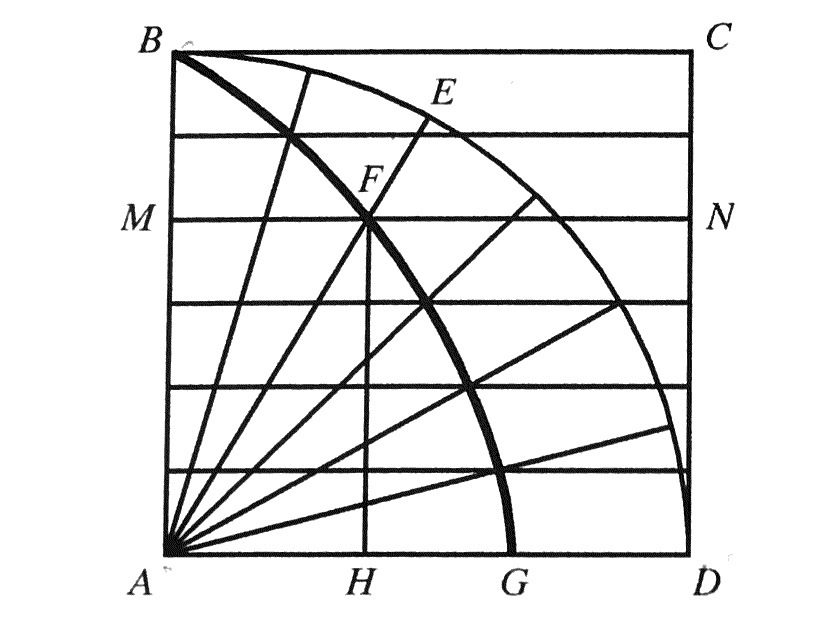
\includegraphics[scale=0.25]{quadratrix.jpg}
\end{center}
	\begin{enumerate}
	\item Use the \emph{definition} of the quadratrix to give a precise mathematical relationship between $\angle EAD$ and line segment $FH.$ 
	\vfill
	\item Explain why Hippias' definition of the quadratrix technically did not contain point $G$ and explain how we define that point in modern terms.\\
	\vfill
	\item Hippias' used the quadratrix for what purpose?
	\vfill
	\item In the historical development of Greek mathematics, the quadratrix was the first example of a curve with what property?
	\vfill
	\end{enumerate}
\newpage

%%%quad of lune
\item (10 points) The questions below concern Hippocrates' Quadrature of a Lune.
	\begin{enumerate}
	\item What is a \emph{lune}?
	\vfill
	\item What is meant by \emph{a quadrature of a lune}?
	\vfill
	\item Why was Hippocrates' quadrature of a lune considered to be a significant result at the time? (To be clear, this questions is asking why Hippocrates' and his contemporaries viewed this result as important. It is not asking for a modern view of the result.)
	\vfill
	\end{enumerate}
%%%Elements as a text
\item (15 points) The following questions concern Euclid's \emph{Elements of Geometry}.
	\begin{enumerate}
	\item Why did the fifth postulate of Book I receive so much attention by so many mathematicians? (Your answer should be limited to the motivation of mathematicians in roughly the first 1000 years after the \emph{Elements} was written.)
	\vfill
	\item With what two propositions does Book I end?
	\vfill
	\item Describe at least two mathematical subjects that appear in the \emph{Elements} other than 2-dimensional plane geometry.
	\vfill	
	\end{enumerate}

\newpage

%%%Archimedes
\item (15 points) The following questions concern the mathematics of Archimedes.
	\begin{enumerate}
	\item Describe the method Archimedes used to estimate the circumference of a circle. You may draw a picture to aid your written description.
	\vfill
	\item Given a circle of diameter 20, assume a mathematician estimates the circumference to be $63\frac{1}{10}$ (i.e. $63.1$). What estimate of $\pi$ does this correspond to?
	\vfill
	\item Describe the method Archimedes used in his quadrature of a parabolic segment. You may draw a picture to aid your written description.
	\vfill
	\end{enumerate}
\newpage

%%%soemthing else about the elements
\item (10 points) Below is a translation of Proposition 9 from Book II of Euclid's \emph{Elements} along with an accompanying figure.
\begin{quote} \textbf{Begin Quote} \\If a straight line is cut into equal and unequal segments, then the sum of the squares on the unequal segments of the whole is double the sum of the square on the half and the square on the straight line between the points of section. \\

Let a straight line $AB$ be cut into equal segments at $C,$ and into unequal segments at $D.$\\

I say that the sum of the squares on $AD$ and $DB$ is double the sum of the squares on $AC$ and $CD.$\\

\textbf{End Quote}
\end{quote}

\begin{center}
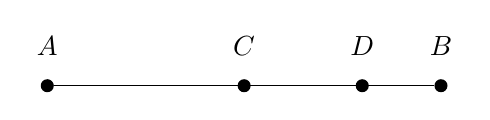
\begin{tikzpicture}
\node[fill,circle,scale=0.5] (a) at (0,0){};
\node[fill,circle,scale=0.5] (c) at (2.5,0){};
\node[fill,circle,scale=0.5] (d) at (4,0){};
\node[fill,circle,scale=0.5] (b) at (5,0){};
\draw (a) -- (b);
\node at (0,0.5){$A$};
\node at (2.5,0.5){$C$};
\node at (4,0.5){$D$};
\node at (5,0.5){$B$};
\end{tikzpicture}
\end{center}

\vspace{.2in}

If $AC=x,$ $CD=y$ and $DB=z$, rewrite the proposition using the symbols $x$, $y$, and $z$ and modern algebraic notation. Then show that this algebraic relationship is true.

\ee
\end{document}
%%%%%%%%%%%%%%%%%%%%%%%%%%
%%%%%%%END
%%%%%%%%%%%%%%%%%%%%%%%%%%


 